\chapter{Проектирование приложения для построения графиков} % тестовове название

Необходимо разработать кроссплатформенное приложение для визуализации графических данных. Приложение должно содержать ввод данных из файла. Данные при необходимости преобразовываются и интерполируются для визуализации в области вывода графической информации. Должно присутствовать несколько форматов отрисовки графиков: двухмерный для функции одной переменной, двухмерный для функции двух переменных в виде тепловой карты, трехмерный для функции двух переменных. Должен быть простой и понятный интерфейс, приложение должно быть доступно и легко в использовании и подходило для людей не имеющих опыта в программировании.
\section{Возможные варианты архитектур приложения} % тестовове название
Существует несколько основных принципиальных архитектур приложений от которых зависит как подход к реализации, так и способ последующей эксплуататции готового продукта. Данный выбор влияет на весь проект в целом и от него зависит стек технологий разработки. Далее следуют варианты архитектур и оценка их релевантности относительно поставленных задач, которые приложение должно решать.
\subsection{Архитектура классического приложения рабочего стола}
Приложения рабочего стола являются достаточно надежным вариантом, так как требует стабильности лишь только от ресурсов пользователя, может работать автономно и позволяет использовать низкоуровневые механизмы для оптимизации под конкретную конфигурацию \cite{24, 25}. Для создания кроссплатформенных приложений существует множетство инструментов разработки интерфейсов, например:
\begin{enumerate}
    \item [1)] технологии QT/QML;
    \item [2)] библиотека GTK+;
    \item [3)] платформа Avalonia.
\end{enumerate}
Данная архитектура подходит для приложений, у которых оптимизация и безопасность стоят на более высокой ступени лестницы приоритетов, чем простота эксплуатации, доступность и удобство пользования для людей, не имеющих опыта в программировании.

\subsection{Архитектура клиент-серверного приложения в сети Интернет}
Веб-приложения имеют ряды ограничений для использования аппаратных ресурсов ввиду их более высокого уровня абстракции. Также они почти всегда требуют доступ к глобальной сети. Однако они всегда нацелены на легкость в использовании, доступность и простоту интерфейсов. Данный вид приложения не требует установки и обновлений, достаточно иметь браузер и подключение к сети Интернет. Но главное преимущество веб-приложений в их стандартизации процесса реализации пользовательского интерфейса с использованием технологий HTML и CSS \cite{27}. Современные приложения рабочего стола, используемые в качестве микросервисов и даже полномасштабных инструментов для редактирования различных видов информации, все больше переходят на архитектуру веб-приложений из-за ее преимуществ в опыте пользователя, например пакет Microsoft Office или Adobe Photoshop. Один из главных минусов данной архитектуры -- зависимость от сервера, на котором расположено приложение: если он выйдет из строя, то никто пользоваться приложением не сможет на время его отключения. Веб-приложения работают на всех платформах одинаково и не требуют отдельных версий. Данная архитектура подходит для небольших сервисов и программ для штучной обработки данных, а также для программ, от которых требуется простой доступ и легкость в использовании. Однако этот вид не подходит для приложений, которые требуют более низкоуровневый подход, оптимизацию и высокую производительность. Данный вид архитектуры отлично подходит для приложения для построения графиков. На рисунке \ref{fig:4} показана визуализация архитектуры клиент-серверного приложения.

\begin{figure}[h!]
    \center
    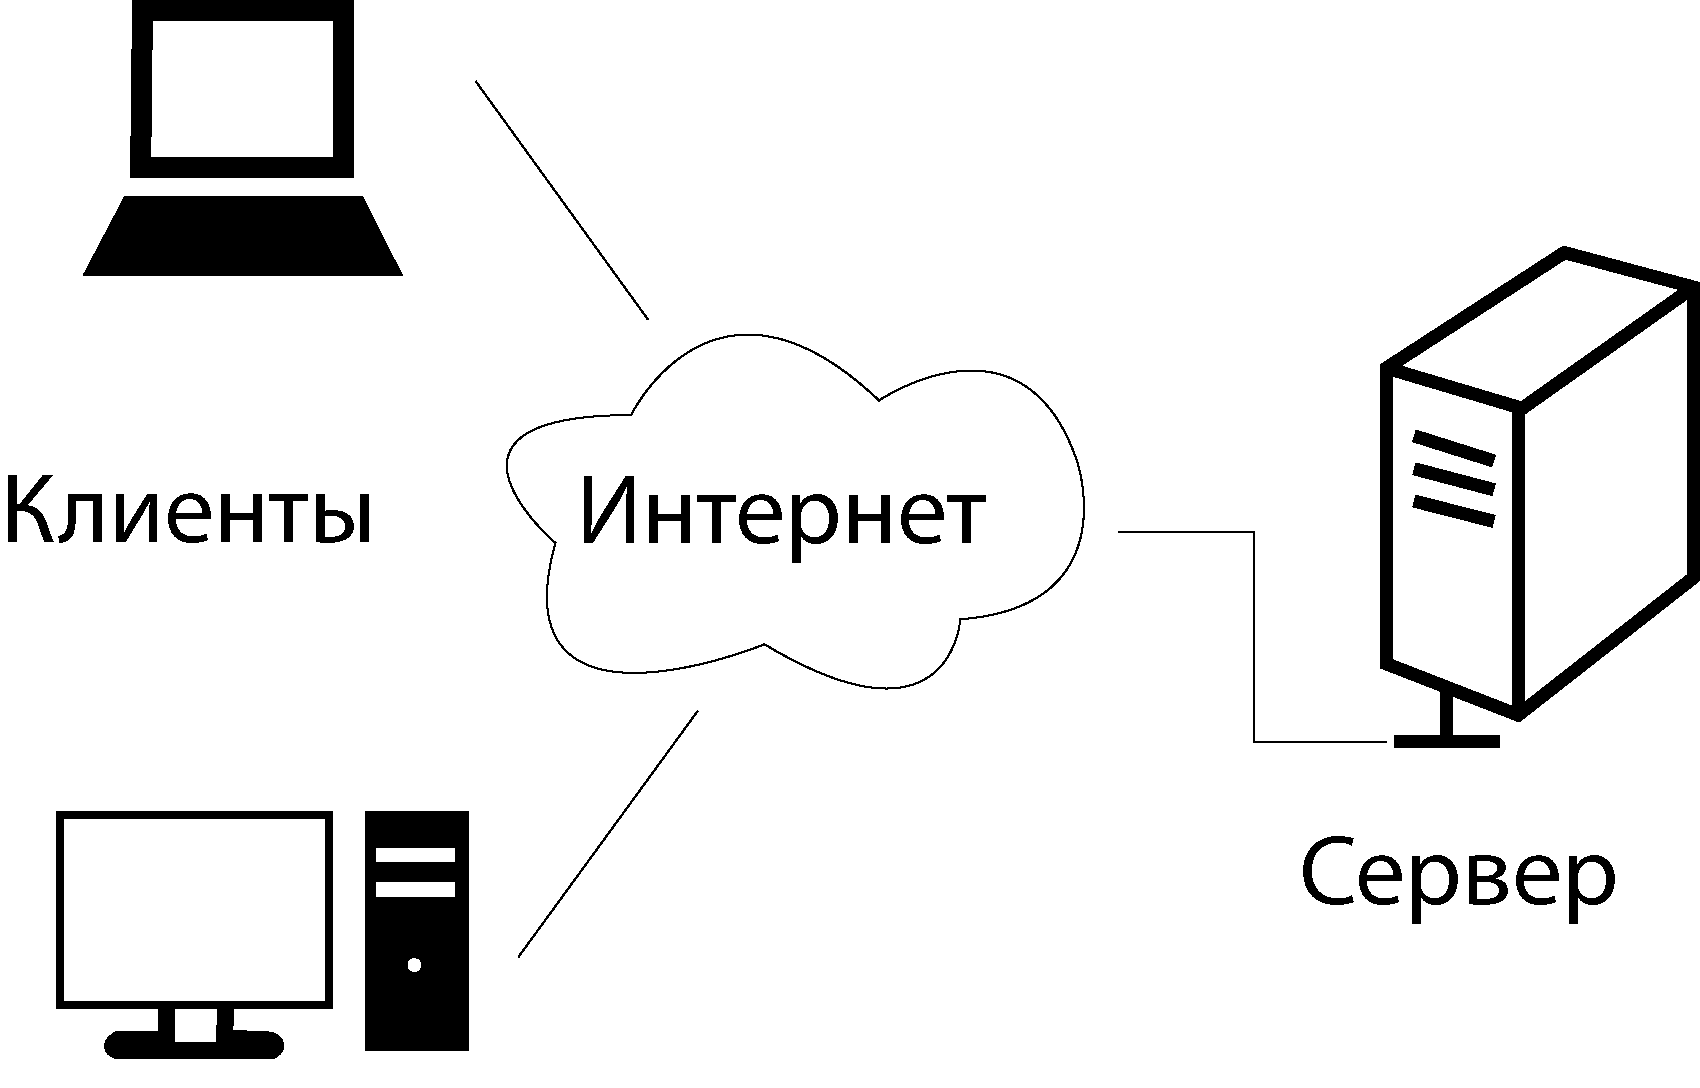
\includegraphics[scale=1]{fig/arc.png}
    \caption{Архитектура клиент-серверного приложения}
    \label{fig:4}
\end{figure}

\subsection{Архитектура приложения рабочего стола с применением технологий разработки клиент-серверных приложений}
Данный вид приложений совмещает преимущества и недостатки предыдущих двух. В данной архитектуре и клиентом и сервером является персональный компьютер пользователя и работает оно в режиме приложения рабочего стола. Однако технологии разработки приложения используются те же, что и для веб-архитектуры. Это позволяет совместить опыт пользователя веб-приложения и автономность работы классического приложения рабочего стола. Кроме того, весь проект реализуется как веб-приложение, в которое добавляется технология перевода его в работу приложения рабочего стола. Некоторые из подобных технологий:
\begin{enumerate}
    \item [1)] фреймворк NW.js;
    \item [2)] фреймворк Electron;
    \item [3)] подход прогрессивного веб-приложения(PWA).
\end{enumerate}
Данные инструменты позволяют создать простое автономное приложение основанное на веб-разработке. Однако этот подход создает малооптимизированное приложение, которое требует много ресурсов. Данная архитектура также подходит для разработки кроссплатформенного приложения для визуализации графической информации, если требуется автономность работы приложения.
\section{Основные функции приложения для построения графиков} % тестовое название

Приложение должно принимать на вход текстовый файл с набором точек, посчитанных программно или записанных вручную, в строковом формате с заданным наперед разделителем. Программа обрабатывает полученные данные, интерполирует их при необходимости и подготавливает к выводу на экран. Программа должна быть способна выводить на экран трехмерную или двухмерную визуализацию поданных на вход объектов. Программа дает возможность выбрать стиль графика и вид его отображения, также должна быть предусмотрена опция масштабирования графика и поворота (для трехмерных графиков). Приложение должно быть кроссплатформенным и иметь простой, интуитивно понятный интерфейс, подходящий  для простого пользователя без опыта программирования. Также необходима функция вывода графического изображения в файл.


\section{Выбор подходящих инструментов разработки для реализации приложения}

Архитектура веб-приложений всегда подразумевает использование для разработки технологии HTML, CSS и JavaScript. Однако способов их использований достаточно много. Существуют готовые библиотеки и фреймворки для веб разработки, которые определяют набор технологий. Самые популярные из них:
\begin{enumerate}
    \item [1)] vue.js;
    \item [2)] angular;
    \item [3)] react.
\end{enumerate}

Все они ускоряют и структурируют разработку и имеют свои преимущества и недостатки, которые в основном влияют на процесс разработки и на этапе проектирования обычно выбор состоит среди их коммерческих лицензий. Для данного проекта с открытым исходным кодом был выбран фреймворк Vue.js так как он является одним из самых простых в изучении. 

Для реализации вывода графиков на экран необходим модуль для работы с графической информацией. Существует несколько библиотек с открытым исходным кодом для работы с графиками, основанными на технологии WebGL среди них: 

\begin{enumerate}
    \item [1)] amCharts.js;
    \item [2)] anyChart.js;
    \item [3)] chart.js;
    \item [4)] d3.js;
    \item [4)] plotly.js.
\end{enumerate}
В качестве серверной основы для веб-приложения будет использоваться Node.js. Среда разработки WebStorm отлично подходит для реализации приложений подобного рода.

\section{Информационная модель проектируемого приложения}
Приложение будет выполнять расчеты интерполяции и рендеринга графика на стороне клиента за счет ресурсов пользователя, за эту часть отвечает модуль визуализации. Интерфейс пользователя реализуется инструментами HTML и CSS. Веб-сервер Node.js отвечает за развертывание приложения, а также для возможности расширения сбора статистики пользователей. Визуализация архитектуры приложения на рисунке \ref{fig:5}.

\begin{figure}[h!]
    \center
    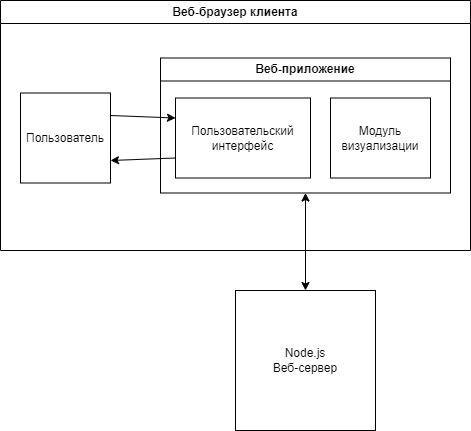
\includegraphics[scale=1]{fig/architechture.png}
    \caption{Архитектура проектируемого приложения}
    \label{fig:5}
\end{figure}

Возможности пользователя отображены на диаграмме вариантов использования, указанной на рисунке \ref{fig:6}. Они смоделированы на основе главного функционала проектируемого приложения. Пользователь может загрузить данные, выбрать параметры визуализации, а именно размерность графика и способ интерполяции, построить график и выбрать для него стиль.

\begin{figure}[h!]
    \center
    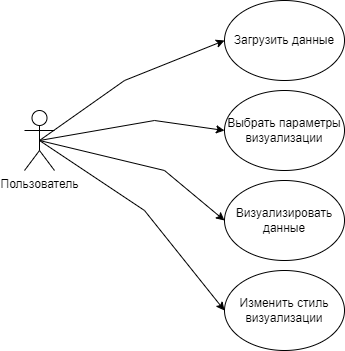
\includegraphics[scale=1]{fig/variant_use.png}
    \caption{Диаграмма вариантов использования проектируемого приложения}
    \label{fig:6}
\end{figure}

На рисунке \ref{fig:7} указана диаграмма взаимодействия.

\begin{figure}[h!]
    \center
    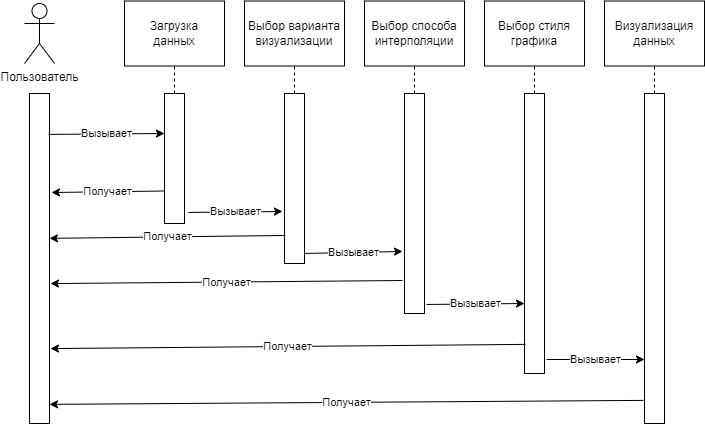
\includegraphics[scale=0.60]{fig/vzaim.png}
    \caption{Диаграмма взаимодействия проектируемого приложения}
    \label{fig:7}
\end{figure}

\newpage
\section{Примеры существующих приложений для построения графиков}

Приложение для построение графиков было спроектировано на основе функционала других приложений. Основные идеи были взяты из двух существующих программ. Первой является Advanced Grapher -- мощный инструмент для визуализации графических данных, а также анализа и исследования функций. К сожалению интерфейс и удобство пользования данной программой достаточно устарели (рисунок \ref{fig:8}). Главной функцией, позаимствованной из данного приложения -- ввод и предобработка данных из файла.

Второй программой, повлиявшей на проектирование архитектуры приложения для построения графиков, является Geogebra.org -- интерактивный инструмент для построения и исследования функций и их графиков. Данная программа выполнена в архитектуре веб-приложения и имеет ряд преимуществ в области пользовательского интерфейса (рисунок \ref{fig:9}). Также она имеет возможность стоить трехмерные поверхности, поворачивать их и масштабировать с помощью мыши. Однако данное приложение не способно построить график по точкам из файла и требует ввода аналитической функции, также оно не поддерживает функции математического анализа для исследования функций.

\begin{figure}[h!]
    \center
    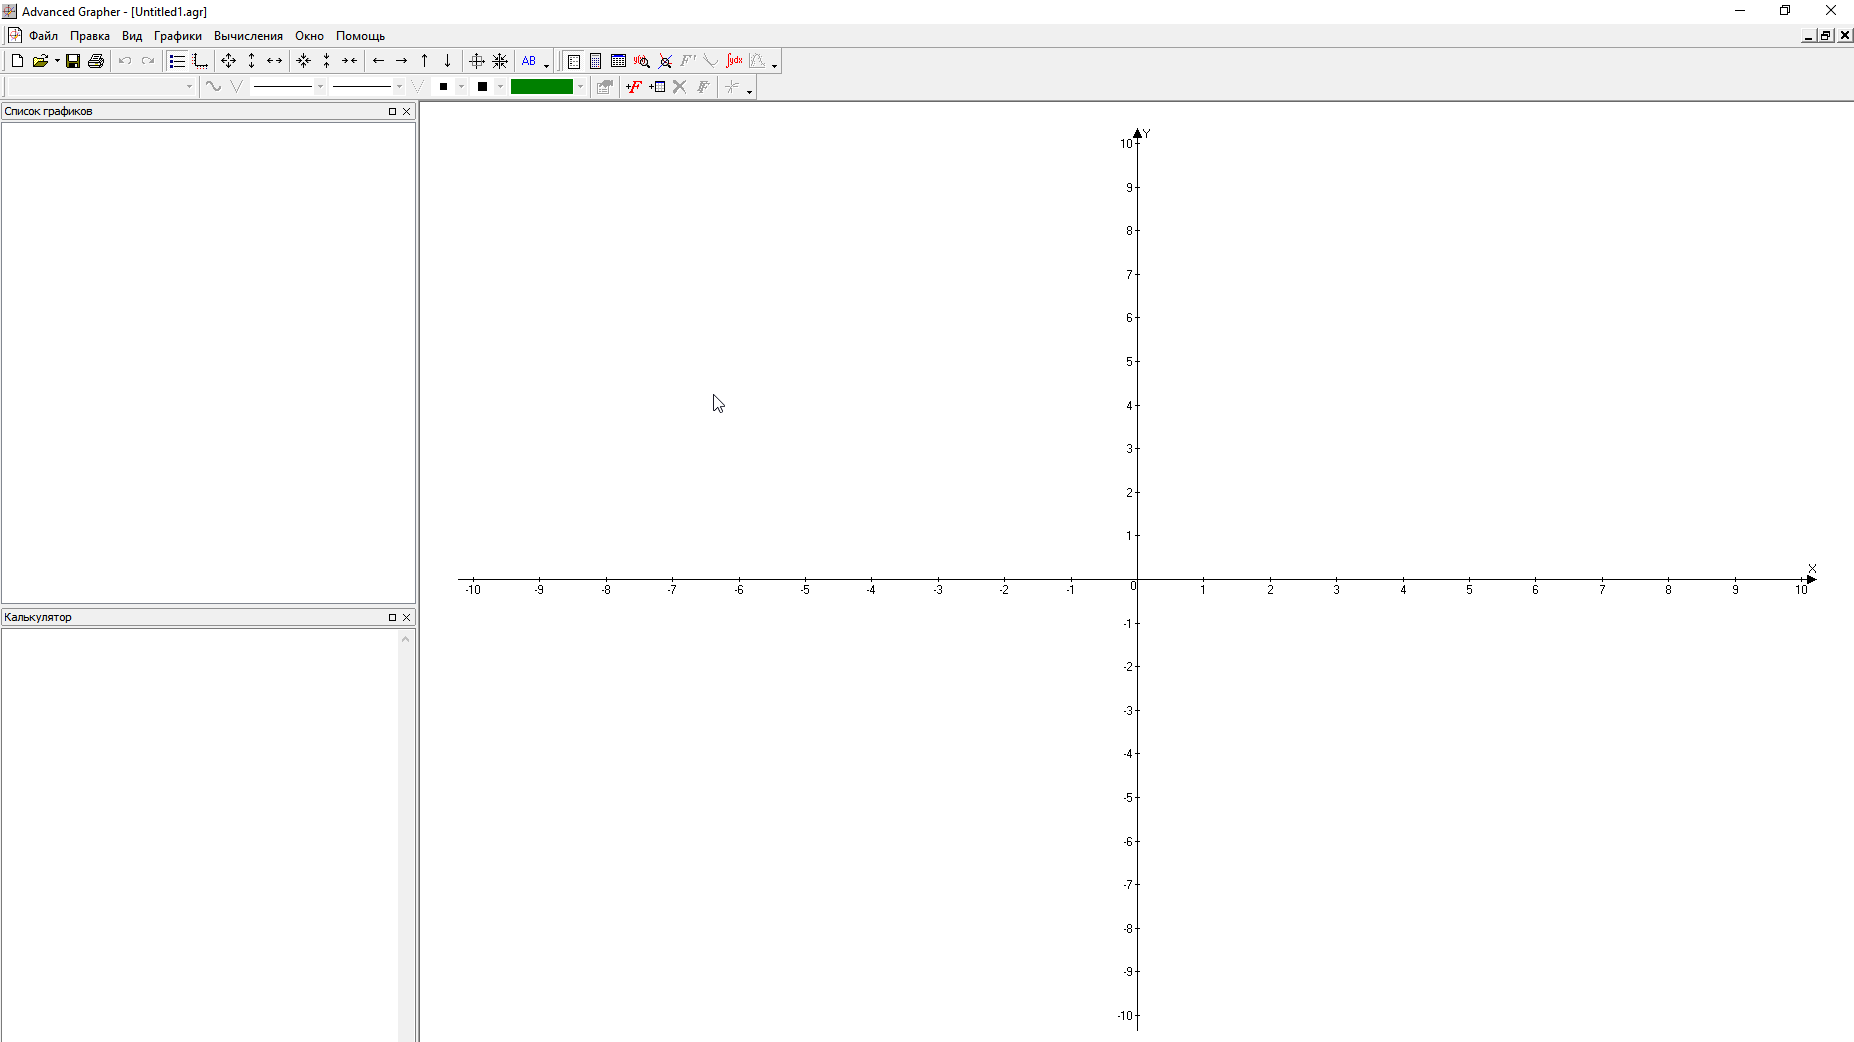
\includegraphics[scale=0.3]{fig/adgrapher.png}
    \caption{Интерфейс приложения Advanced Grapher 2.2}
    \label{fig:8}
\end{figure}

\begin{figure}[h!]
    \center
    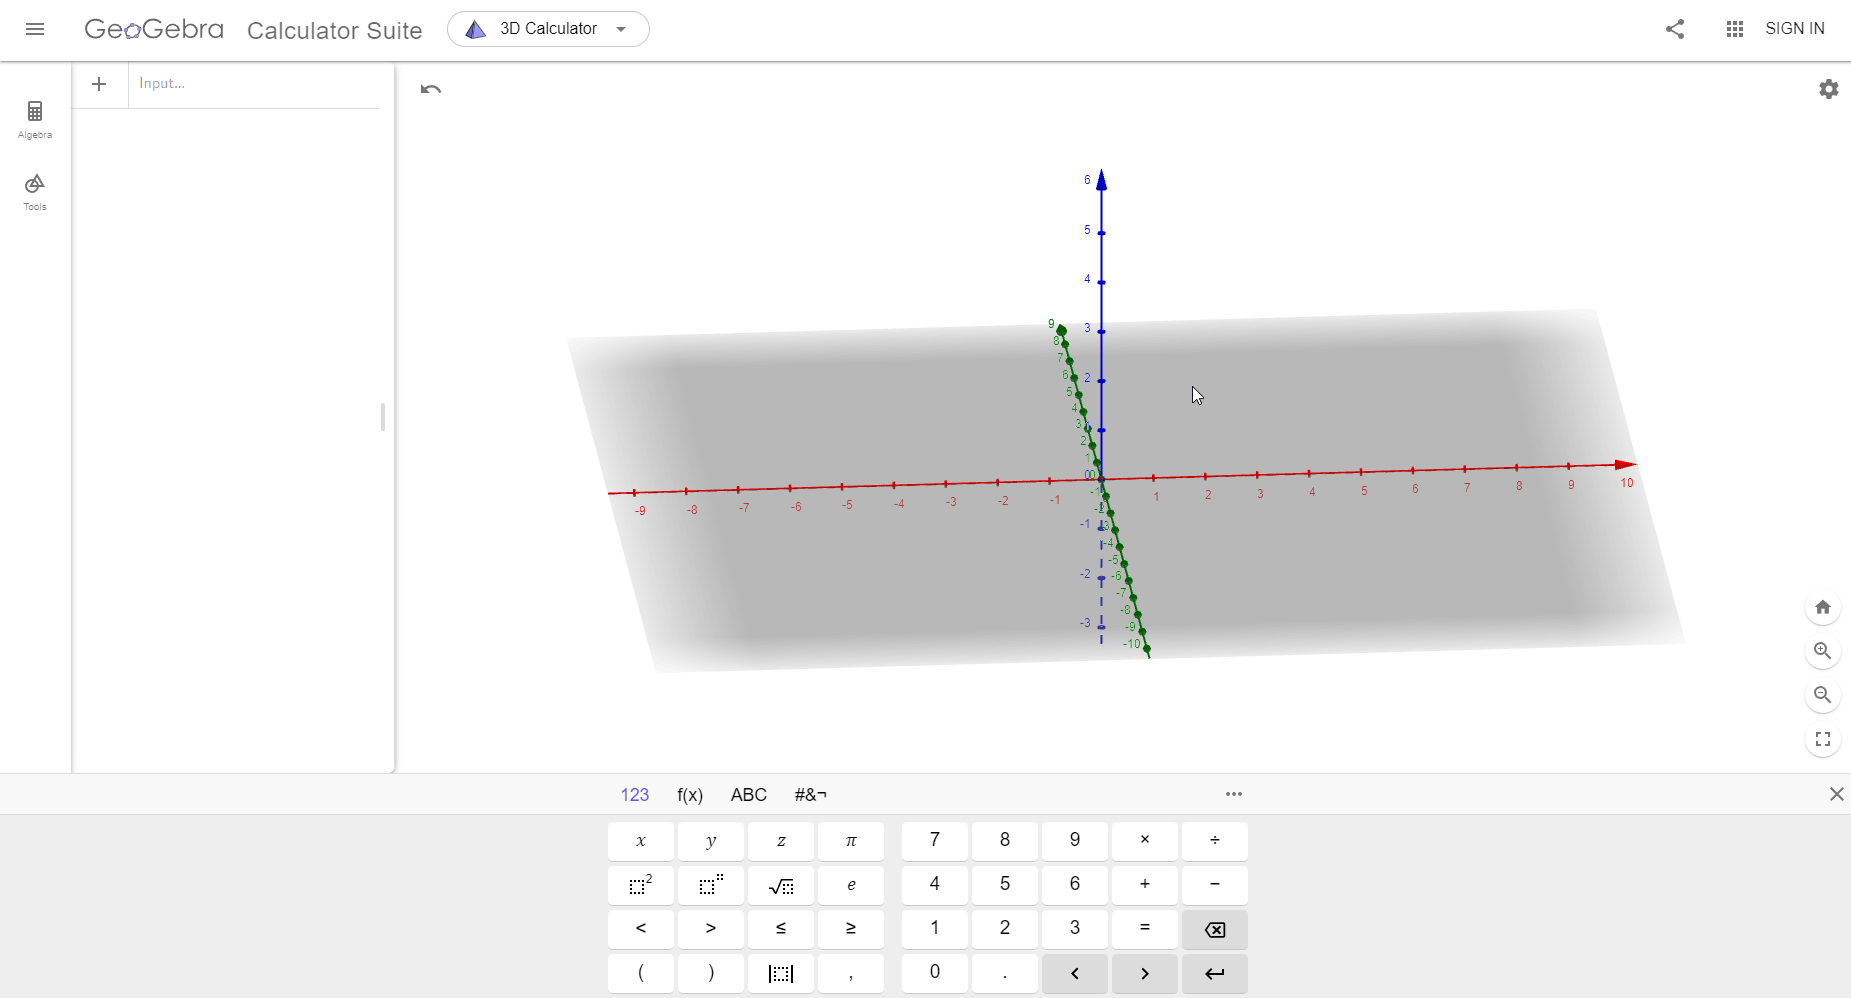
\includegraphics[scale=0.3]{fig/Geogebra.png}
    \caption{Интерфейс приложения Geogebra.org}
    \label{fig:9}
\end{figure}

Интерфейс проектируемой программы будет схож с решением от программы Geogebra, предполагается иметь элемент ввода текстового файла с данными, область отображения графической информации, а также блок настроек визуализации и стиля графиков. На рисунке \ref{fig:10} изображено ориентировочное расположение элементов интерфейса проектируемого приложения.

\begin{figure}[h!]
    \center
    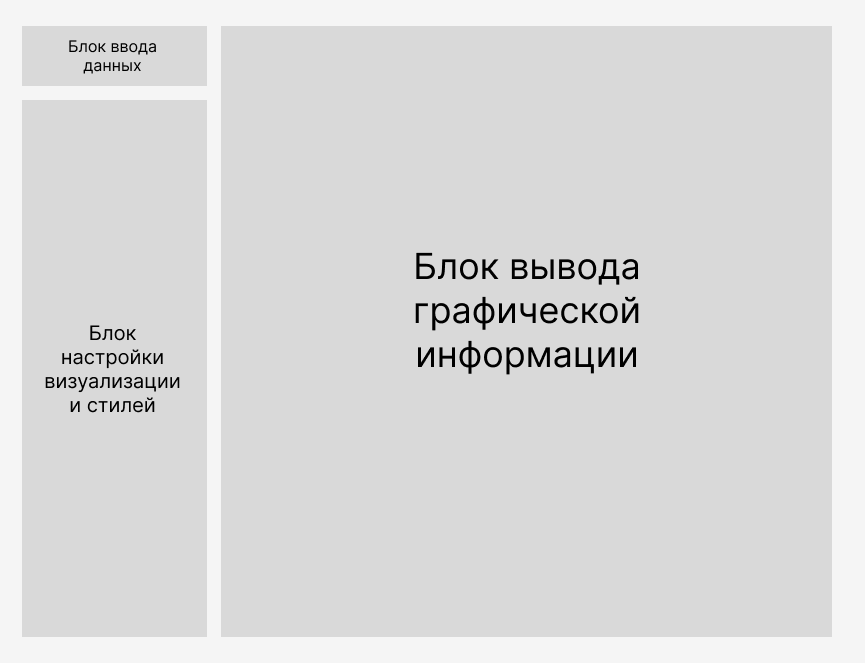
\includegraphics[scale=0.7]{fig/interface_prototype.png}
    \caption{Прототип интерфейса для приложения для построения графиков}
    \label{fig:10}
\end{figure}